\documentclass[usenames,dvipsnames]{article}

\usepackage{tikz-feynman}
\usepackage{xcolor}

\begin{document}
    

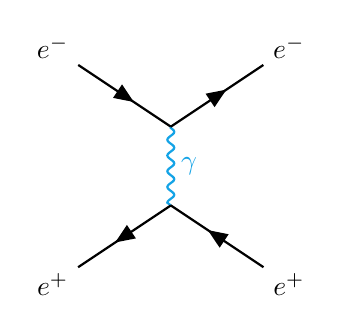
\begin{tikzpicture}
    \begin{feynman}[large]
        \centering
        \vertex (ein) {$e^-$}; % h at beginning 
        \vertex [right=3cm of ein] (eout) {$e^-$}; % h -> ZZ vertex
        \vertex [below right=1cm and 1.5cm of ein] (phot);
        \vertex [below=1cm of phot] (photb);
        \vertex [below=3cm of ein] (pin) {$e^+$}; % h -> ZZ vertex
        \vertex [right=3cm of pin] (pout) {$e^+$}; % h -> ZZ vertex
        \diagram* {
            (phot) -- [boson, edge label=$\gamma$, color=Cerulean] (photb),
            (pout) -- [fermion] (photb) -- [fermion] (pin);
            (ein) -- [fermion] (phot) -- [fermion] (eout);
            };
    \end{feynman}
\end{tikzpicture}

\end{document}